\chapter{Literature Study}
\label{cha:litreview}
In this chapter contains a review of some of the most important techniques necessary to build an end-to-end speech recognition system. After looking at possible input feature representations, the most important machine learning tools will be explored. Finally sequence-to-sequence labeling methods such as CTC and the listen attend and spell architecture are covered.

\section{Preprocessing and feature extraction}
\subsubsection{Filter-Bank features}
\begin{figure}
\centering
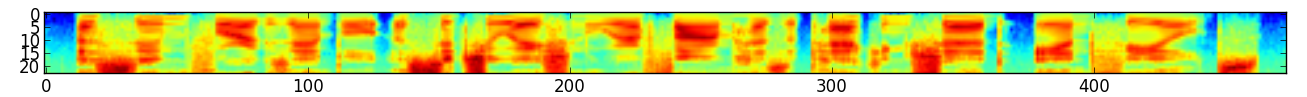
\includegraphics[width=1.0\linewidth]{/png/timitInput}
\caption{Frequency Bank input computed from a sentence contained in the \textit{TIMIT} dataset. Time is shown on x and Frequency on the y-Axis.}
\label{fig:timitInput}
\end{figure}
Filter-banks are collections of filters. These filters can be spread out over audible frequencies\footnote{Approximately 16 to 16000 Hz.}. Filter-bank output is commonly used as input for speech analysis \cite{Huang2001}\cite{Chan2015}. The number of filter-banks depends on the required resolution, 32 is a common choice \cite{Juang1987}. The energy within the part of the signal spectrum described by all individual filters is measured. Figure~\ref{fig:timitInput} shows the resulting energy measurements using 23 filters, for a sentence recording contained in the \textit{TIMIT} data set.
The general argument for filter banks in speech recognition is that the cochlea, in the human ear, resembles a filter bank \cite[page 30]{Huang2001}. Humans do not perceive frequency linearly. Experimental evidence suggests, that our perception of is scaled according to the Mel-Scale \cite[page 34]{Huang2001}:
\begin{equation}
B(f) = 1125 ln(1 + f / 700)
\end{equation}
A normalized plot of this function is shown in figure~\ref{fig:mel} on the left.
According to the Mel-scale, humans are able to distinguish more lower frequencies than higher frequencies. In the plot the first four thousand Herz occupy roughly eighty percent of the scale. The band from four thousand to eight thousand Herz is left with only about twenty percent of the scale, even tough half of the considered frequencies are in this band.
\begin{figure}
\centering
\includestandalone[width=6cm]{tikz/melScale}
\includestandalone[width=6cm]{tikz/melBank}
\caption{The Mel-scale (blue) with Mel-Frequency Cepstrum Coefficients (red)  on the left. Filterbank with Mel-spaced filters (right).}
\label{fig:mel}
\end{figure}
Mel spaced filter-banks are an attempt to include the human perception in speech recognition. The filter functions are defined by \cite[page 317]{Huang2001}:
\begin{align}
H_m &= 0 									   &\text{if}\;\; & k < f[m-1] \\
H_m &= \frac{k      - f[m-1] }{f[m] - f[m-1]}  &\text{if}\;\; & f[m-1] \leq k \leq f[m] \\
H_m &= \frac{f[m+1] - k      }{f[m + 1] - f[m]}&\text{if}\;\; & f[m] \leq k \leq f[m+1] \\
H_m &= 0									   &\text{if}\;\; & k > f[m+1]
\end{align}
In the equations above $H_m$ denotes the magnitude of filter $m$ with a total of $M$ filters. The frequency is denoted by $k$, the vector $f$ contains $M+2$ linearly spaced filter border values. These are the red stars on the left of  figure~\ref{fig:mel}. The right plot shows the triangular filter banks. These banks are spaced according to the same values. Roughly speaking using mel-filter banks means using a high filter resolution where human hearing is good and a low resolution where it is bad. \\
In addition to perceptually motivated instantaneous features, derivative information can be appended to each feature vector. These so called delta features add information
regarding the speed of change taking into account $2*N$ feature vectors. $N$ denotes the number of frames back and forward in time. The derivative information can be computed using \cite{Woodland2006}. The mel feature vectors are denoted by $\mathbf{c}$:
\begin{equation}
\mathbf{d}_t = \frac{\sum\limits_{n=1}^{N} n (\mathbf{c}_{t+n}- \mathbf{c}_{t-n})}{2 \sum\limits_{n=1}^{N} n^2}
\end{equation}
The formula above is a central difference, because the value at time t is not taken into account, in contrast to forward or backward differences, where the value at t is part of the difference. A common choice for $N$ is two. In this case the formula above simplifies to:
\begin{equation}
\mathbf{d}_t = \frac{2\mathbf{c}_{t+2} + \mathbf{c}_{t+1} - \mathbf{c}_{t-1} - 2\mathbf{c}_{t-2}}{10}
\end{equation}
In this case two future frames are used to compute the derivative at time $t$, which implies, that at computation time a full recording is available. Should that not be the case a backward difference scheme should be considered instead. To further augment the features second derivative or acceleration information can be added as well. These can be computed by simply applying the central difference to the deltas one more time. It is important to note that augmenting the features with derivative information significantly increases their dimension. If 40 mel-filters are used then the first and second derivatives will contain 40 entries each, therefore increasing the input dimension from $40$ to $120$.

Before using the features it is best practice to standardize the components of the input vectors. It is desirable to use features with an overall mean of zero and a standard deviation of 1 over the entire training set \cite[page 30]{Graves2008}. The feature normalization process starts by computing the mean,
\begin{equation}
\mathbf{m}_i = \frac{1}{\|S\|} \sum\limits_{\mathbf{x} \in S} \mathbf{x}_i
\end{equation}
and standard deviation
\begin{equation}
\sigma_i = \sqrt{\frac{1}{|S| - 1}\sum\limits_{x \in S}(\mathbf{m}_i - \mathbf{x}_i)^2}
\end{equation}
Of a data set $S$ consisting of input $\mathbf{x}$ and target $\mathbf{t}$ pairs. Standardized input vectors can then be computed using:
\begin{equation}
\hat{\mathbf{x}}_i = \frac{\mathbf{x}_i - \mathbf{m}_i}{\sigma_i} \text{  for all } \mathbf{x}_i \in S.
\end{equation}
Input standardization is beneficial to network performance, because it puts the input values in ranges, which standard activation functions such as sigmoids or hyperbolic tangents can handle better \cite[page 30]{Graves2008}.

Mel-Frequency banks are considered high level feature inputs. When the recognition system is found to work with these, features on a lower level or even raw data could be used as input. The idea behind doing less preprocessing, is that the network might be able to come up with something better on its own.

\section{Neural Networks}
Artificial neural networks where originally designed to model biological neurons. Even tough it is now known that artificial neural networks have little in common with their counterparts in biology, the models are still popular due to their useful pattern recognition properties \cite[page 13]{Graves2008}. All neural networks consist of elementary functions with weighted and biased inputs, the operations necessary to evaluate them form a computational graph. In a nutshell the idea is to choose the weights and biases such that the network output corresponds to patterns seen in the input data. The process of finding good weights is called training. Training in turn is done using gradient descent.

\subsection{Gradient descent}
The optimization process of neural networks works with a training data set $\{\{\mathbf{x}_1,\mathbf{t}_1\}$, $\dots ,$ $\{\mathbf{x}_p,\mathbf{t}_p\} \}$ \cite[page 156]{Rojas1996}. The elements of this set are the input- and output-patters $\mathbf{x}$ and $\mathbf{t}$ respectively. For each input vector the network output $\mathbf{o}$ is computed. Ideally the network output should be the same as the desired target $\mathbf{t}$ one for all data pairs. The difference between target and current outputs could be measured by the cost function \cite[page 156]{Rojas1996}:
\begin{align}
E = \frac{1}{2}\sum\limits_{i=1}^{p} \| \mathbf{o}_i - \mathbf{t}_i \|^2.
\end{align}
However generally the more complex cross-entropy is used as a cost function, because it leads to faster convergence and better results in practice \cite{Golik2013}. For classification tasks, cross entropy is defined as \cite[page 245]{Bishop1995}:
\begin{equation}
E = - \sum\limits_{i=1}^{p} {\mathbf{t}_i \ln(\mathbf{o}_i)} + (1 - \mathbf{t}_i)\ln(1 - \mathbf{o}_i)
\label{eq:corssEntropy}
\end{equation}
In order to understand why the cross entropy is a measure of output error, the two scalar cases $t=0$ and $t=1$ are considered. For $t = 0$ the cross entropy simplifies to $-\ln(1 - o)$. Looking at figure~\ref{fig:logPlot}, this expression turns out to be a good cost function, because for values close to the desired output $o = 0$, $-\ln(1 - o)$ will be close to zero. If the output moves away from the desired value zero, the cost grows asymptotically. If $t = 1$ is considered the cost function simplifies to $-\ln(o)$ which will be zero for the desired output and once more displays asymptotic growth for undesired values far away from one. If the target probability is somewhere between these two extreme cases the cost will be the sum of the two cases considered earlier. Cross entropy is statistically motivated, the output vectors $\mathbf{o}$ describe probability distributions over the possible labels, their elements must therefore be $\in (0,1)$ and sum op to one.
\begin{figure}
\centering
\includestandalone[width=6cm]{tikz/logPlot}
\caption{Plot of $y = -\ln(x)$ for $x \in (0,1)$.}
\label{fig:logPlot}
\end{figure}

During the training process a local minimum of the error function $E$ is sought. At this minimum the difference between the network output $\mathbf{o}$ and the target values $\mathbf{t}$ is small. This value might not be the smallest possible value, termination can happen at the global or a local minimum.
After the training process has completed the network is expected to identify similarities to data seen during the training process and produce a similar output.
In order to reach a local minimum, the gradient of the error function is needed. The key idea of gradient descent is to follow the negative gradient until a local minimum is reached.
Neural networks can be considered as large composite functions, which are made up of elementary operations. The evaluation of the network can be written as a graph. Computations are done at each node and information travels trough the network along directed edges from node to node. In order to create a computational graph for the training process each of the output units of the network under consideration are connected to a new node which computes $\frac{1}{2}(o_{ij} - t_{ij})^2$\cite[page 157]{Rojas1996} or the cross-entropy term of one data target pair. These new nodes in turn are connected to one more node, which sums up all error values and produces $E_i$. The process described above must be repeated for all training data pairs. One final node is added, which sums up all values $E_i$. Its output gives the value for the error function $E$ which is now in the form of a large graph.\\
Reverse mode algorithmic differentiation or back-propagation is an algorithm to compute the gradient of a graph consisting of basic elementary operations. As an example its operation is now illustrated using the function \cite[page 69]{Diehl2013}:
\begin{align}
f(w_1,w_2,w_3) = \sin(w_1 w_2) + \exp(w_1 w_2 w_3)
\label{eq:backFun}
\end{align}
This function written in terms of five elementary operations as \cite[page 70]{Diehl2013}:
\begin{align}
w_4 = w_1 w_2 \\
w_5 = sin(w_4)\\
w_6 = w_4 w_3 \\
w_7 = exp(w_6) \\
w_8 = w_5 + w_7 \\
o = w_8
\end{align}
Computing the gradient means computing the partial derivatives of $f$ with respect to all inputs. In this case this means finding:
\begin{align}
\frac{\partial f(w_1,w_2,w_3)}{\partial w_1} = w_2 (\cos(w_1 w_2) + w_3 \exp(w_1 w_2 w_3)) \\
\frac{\partial f(w_1,w_2,w_3)}{\partial w_2} = w_1 (\cos(w_1 w_2) + w_3 \exp(w_1 w_2 w_3)) \\
\frac{\partial f(w_1,w_2,w_3)}{\partial w_3} = w_1  w_2 \exp(w_1 w_2 w_3)
\end{align}
Above the derivatives have been found by hand using the chain rule. Now these will be computed using back-propagation. Figure~\ref{fig:networkGraph} shows a graphical representation of equation~\ref{eq:backFun}. The partial derivatives needed for the backwards sweep can be found on the edges. \\
\begin{figure}
\centering
\includestandalone[width=12cm]{tikz/gd_exampleNet}
\caption{Example funciton network with partial derivatives.}
\label{fig:networkGraph}
\includestandalone[width=12cm]{tikz/gd_reverseSweep}
\caption{Reverse sweep.}
\label{fig:reverseSweep}
\end{figure}
The gradient is computed using a forward and backward sweep. During the forward sweep the inputs are fed into the network and the functions at each node are evaluated layer by layer, until the output at the last node is known. In figure~\ref{fig:networkGraph} this means computing $w_4$ to $w_8$. \\
After the forward sweep the gradient is found by going back trough the network from the output to each input node. Using a seed value of $1$ at the output node the lower unit values are computed by multiplying the associated partial derivative found on each edge. If a node has more then one incoming value, their sum is computed. The process is illustrated in figure~\ref{fig:reverseSweep}. At the roots of the tree the partial derivatives of the output with respect to each input can be found. Together these root values make up the gradient.
To be able to perform the first forward sweep the network weights are initialized at random. The training data pairs are known and can be added as constants to the graph.
If the weights of the network are stored in a weight vector $\mathbf{w}$ the value of the gradient after the $n$th update may be written as \cite[page 27]{Graves2008}:
\begin{equation}
\triangle \mathbf{w}(n) = -\alpha \frac{\partial f}{\partial \mathbf{w}(n)}.
\end{equation}
Where $\alpha \in [0,1]$ denotes the learning rate. Unfortunately simple gradient descent tends to get stuck in local optima. In order to increase the chance of gradient descent to escape from such a local minimum a momentum term can be added to the formulation \cite[page 267]{Bishop1995}\cite[page 27]{Graves2008}:
\begin{equation}
\triangle \mathbf{w}(n) = m\triangle \mathbf{w}(n-1) -\alpha \frac{\partial f}{\partial \mathbf{w}(n)}.
\end{equation}
Above $m \in [0,1]$ denotes the momentum. In order to understand the effect of the momentum term consider a weight space region of very low curvature, where it can be assumed, that the gradient stays constant. Using the momentum formula above yields \cite[page 267]{Bishop1995}:
\begin{align}
\triangle \mathbf{w}(n) &= -\alpha \frac{\partial f}{\partial \mathbf{w}} (1 + m + m^2 + \dots) \\
						&= -\frac{\alpha}{ 1 - m}\frac{\partial f}{\partial \mathbf{w}}.
\end{align}
Using the fact that the sum of the geometric series is known and $|m| < 1$ must hold. The momentum term therefore changes the effective learning rate from $\alpha$ to $\frac{\alpha}{ 1 - m}$ in regions of low curvature. Elsewhere the gradient is oscillatory, which leads to cancellation of successive contribution of the momentum term \cite[page 267]{Bishop1995}.

\subsection{Regularization}
The optimization process works on the training set, but later the trained network should be able to recognize patterns seen in the training data set in other inputs and produce similar outputs. In order to achieve this goal it is important not to memorize training data samples. Another problem with complex networks is that they are able to track noise in the training data.
Regularization techniques aim to counteract sample memorization and noise tracking in order to ensure that progress on the training data carries over to new data sets or in other words regularization aims to improve generalization.

\subsubsection{Early stopping}
The idea of early stopping is to observe the training and validation loss during training. As long as both are falling simultaneously, we assume that
the network will also generalize well to other data. This is a reasonable assumption, because the validation data set plays no part in computing the weight updates. When the training set loss continues fall, but the validation loss rises, the network is overfitting \cite[page 31]{Graves2012}. The training process should be stopped early in theses cases.
A test set should be used to guard against parameter choices that work well only on the training and validation set. Ideally the performance on the test set should only be evaluated, once the training process has finished.

Care must be taken, when dividing the entire data set into training, validation and test subsets. All three sets must be good representations of the overall data set. Differences for example regarding the noise level should be avoided. Furthermore the sizes of all sets must be chosen carefully. Using too few samples for validation and testing, makes it very hard to guard against over-fitting. If the training set becomes to small, overall performance might suffer. In practice a good trade off must be found experimentally.

When data collection is expensive cross validation should be used. Cross validation divides the merged training and validation data sets into $k$ subsets. During each iteration one of the $k$ subsets is used for validation and the remaining $k-1$ sets are used for training. Cross-validation has the advantage that each subset is used for training and validation, thus making more efficient use of the total data set. The test set is very important when working with cross validation, because the validation data is part of the training process. It should be sufficiently large to detect over-fitting.
  

\subsubsection{Input Noise}
Training with input noise means that fixed variance, zero mean Gaussian noise is added to the inputs during training \cite[page 32]{Graves2012}. The targets remain unchanged. The idea is to reuse the training data set more efficiently. When the artifical noise is similar to the noise already present in the data set, reusing the noisy samples is better than reusing the original samples. Input noise decreases the reliability of the inputs during training, is covers small variations caused by noise in the data, which the network could remember without it during training, if the noise was not present. Furthermore the artificial noise will help the network to deal with similar noise in the future, making the trained system more robust. 
A problem with input noise is that it is difficult to determine how large the variance should be, one option is to manually tune the parameter using the validation performance as a metric.

\subsubsection{Weight noise}
When using weight noise zero mean fixed variance Gaussian noise is added to the weights during training. The idea is to reduce the precision, with which the network weights can be described \cite[page 32]{Graves2012}. The reduced precision makes it impossible for the network to model small variations in the training samples, which are likely to be noise. Instead it will only be able to model larger changes and generalize better.
When using input noise the following algorithm should be used \cite[page 33]{Graves2012}:
\begin{lstlisting}[language=python]
while stopping condition is False:
    Shuffle training data pairs
    for each training sample pair:
        Add Gaussian noise to weights
        compute the gradient
        restore original weights
        update the original weights
\end{lstlisting}
However weight noise should be used with care, because it can lead to very slow convergence.

\subsubsection{Regularized loss minimization}
Regularized loss minimization includes a model complexity penalty term in the cost function. Instead of minimizing the loss $E$ an augmented loss \cite[p. 338]{Bishop1995}\cite[p. 171]{Ben-david2014}:
\begin{equation}
\hat{E} = E + v\Omega
\end{equation}
is used. $\Omega$ stands for a penalty term, which should grow, when the network is likely to over-fit the training data. $v \in (0,1)$ denotes the weight parameter, which determines how much emphasis the optimization algorithm should place on regularization. A straightforward choice for $\Omega$ is the $l_2$ norm of the model weights:
\begin{equation}
\Omega_{l2} = \|\mathbf{w}\|^2 = (\sqrt{ \sum w^2})^2
\end{equation}
The weight norm serves as a measure for the model complexity. The idea of choosing the simplest possible model which can explain the data, often referred to as Occam's razor is expressed in the modified cost function $\hat{E}$, the result of the optimization process will be a compromise between fit to the training data and model complexity.


\subsubsection{Dropout}
\begin{figure}
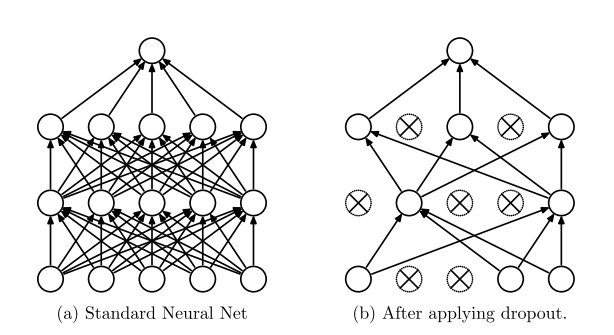
\includegraphics[width=1.0\linewidth]{/png/dropout}
\caption{\enquote{Dropout Neural Net Model. Left: A standard neural net with 2 hidden layers. Right: An example of a thinned net produced by applying dropout to the network on the left. Crossed units have been dropped.} \cite{Srivastava2014}, image and caption taken from the same source.}
\label{fig:Dropout}
\end{figure}
Like input noise and weight noise dropout is part of the group of regularization techniques, that artificially corrupt training data to improve prediction performance \cite{Wager2013}. When applying dropout between two layers, some units and their connections are zeroed out at random during training. The process is illustrated in figure~\ref{fig:Dropout}.
One dropout interpretation relates dropout networks to committee networks. Network committees consist of several independently trained networks, each of which makes predictions on its own. The committee prediction is then produced by using the mean output of the committee members or by feeding the committee outputs into another neural net, which decides on the final output.
When training large deep networks however committee networks become infeasible due to their large memory requirements. Dropout networks are related to committee networks, because when some units are dropped the remaining units will have to learn to work with the remaining units. Just like committee networks, dropout networks contain multiple mechanism to recognize the same pattern, and thus gains some of the prediction robustness that committee networks are know to have.
Another motivation for dropout comes from the theory of sexual selection \cite{Srivastava2014}. The theory assumes that the superiority of sexual reproduction is caused by the fact that removes strong interconnections between genes. After all a specific gene might not be there a generation from now. To function over many generations, genes must therefore develop redundant ways that work with different genes.
Following this interpretation dropout forces network units to do the same thing.

\subsection{Deep Neural Networks}
Deep learning deals with the design of computational nets, consisting of multiple layers, which learn representations of data. Deep networks are often used when abstract
patterns must be found. Simple networks are often unable to cope with the problem complexity, and fail to recognize the underlying structure. Human speech features such complex patterns, therefore deep networks must be considered. Increasing the network depth leads to many additional weights, for which a suitable value must be found.
In addition to the added memory load caused by the extra weights, the optimization process must look trough large data sets until a suitable optimum is reached.
\subsubsection{Stochastic gradient descent}
When training deep  networks on very large data sets, working with the full data set to compute the current gradient becomes very inefficient. It is common practice to use stochastic gradient descent instead of the classic algorithm. The idea is to select small subsets of the full data set. These so called mini-batches are then used to compute the outputs and errors, as well as the gradients for these smaller examples. Instead of working with the gradient of the union of these mini-batches the average gradient is computed and used to update the network weights. This approach dramatically reduces the memory requirements of the training process, which makes it possible to work with more sophisticated network designs.

\subsection{Recurrent Neural Networks}
\begin{figure}
\centering
\includestandalone[width=7cm]{tikz/recurrentCell}
\caption{Visualization of a single recurrent cell.}
\label{fig:singleRecCell}
\includestandalone[width=9cm]{tikz/recNet}
\caption{Rolled (left) and unrolled (right) recurrent neural net with two units.}
\label{fig:unrolledNet}
\end{figure}
When processing speech its is important to take context into account. When spelling the letters which make up a word, it is important to know what the previous letter was, in order to make the right decision.
Feed-forward neural nets do not possess memory. These networks make decisions, starting from zero every time. In oder to fix this a cell state variable can be introduced. A simple recurrent cell where the current state is set to the previous output is shown in figure~\ref{fig:singleRecCell}. Another way to depict the same architecture is shown in Figure~\ref{fig:unrolledNet}, here the cell state is not labeled explicitly, the single cell on the left is just a simplified version of the figure above. If the network is unrolled in time the flow of the state becomes apparent, which is done in figure~\ref{fig:unrolledNet} on the right.
The unrolled form shows a direct dependency of the output at time $t$ on the previous output at $t-1$, which in turn depends on the previous outputs. This causes $y_t$ and $y_{t-1}$ to change together. In other words: The introduction of recurrent connections leads to correlation of the two outputs.


\subsubsection{The exploding and vanishing gradient problem}
Even tough past information is available in theory, RNNs have only limited access to contextual information in practice \cite[page 1]{Graves2008}. Due to problems with gradient descent on correlated data, the back-propagated derivative can sometimes become weaker and weaker until it ultimately vanishes \cite{Hochreiter1998}. Another problem is that sometimes classical recurrent neural nets produce a gradient that blows up \cite{Pascanu2012}. The exploding gradients can be fixed by clipping, but vanishing gradients require more sophisticated treatment \cite{Bengio1993}.

\subsubsection{Long short-term memory}
Initially researchers tried to solve the vanishing gradient problem by making changes to the training algorithm using simulated annealing, time delays or compression \cite[page 32]{Graves2008}. However a good solution to the problem turned out to be changing the RNN cell architecture. Long short-term memory (LSTM) cells as proposed in \cite{Hochreiter1995} are more complex network units. LSTMS are differentiable versions of memory chips in a digital computer. Memory chips generally have read, write, and erase ports which can be set in order to allow the chips state to be read, modified or emptied. In the LSTM case the input, output, and forget gates serve the same function \cite[page 33]{Graves2008}. Throughout the literature these gates are generally denoted as $\mathbf{i}, \mathbf{f}$ and $\mathbf{o}$. The content of the memory or state is written as $\mathbf{c}$, the output as $\mathbf{h}$, while a $t$ subscript denotes the time step.
These memory cells use the differentiable equation system \cite[page 5]{Graves2013}\footnote{ Various versions of LSTM cells exist. This one is commonly referred to as the \textquotedblleft peephole\textquotedblright $ \: $ variant. }:
\begin{align}
\mathbf{i_t} &= \sigma (\mathbf{W}_{ix} \mathbf{x}_t + \mathbf{W}_{ih} \mathbf{h_{t-1}} + \mathbf{W}_{ic} \mathbf{c_{t-1}} +\mathbf{ b}_i) \\
\mathbf{f_t} &= \sigma (\mathbf{W}_{fx} \mathbf{x}_t + \mathbf{W}_{fh} \mathbf{h_{t-1}} + \mathbf{W}_{fc} \mathbf{c_{t-1}} +\mathbf{ b}_f) \\
\mathbf{c_t} &= \mathbf{f_t} \mathbf{c_{t-1}} + \mathbf{i_t} \tanh( \mathbf{W}_{cx} \mathbf{x}_t + \mathbf{W}_{ch} \mathbf{h_{t-1}} + \mathbf{b}_c ) \\
\mathbf{o_t} &= \sigma (\mathbf{W}_{ox} \mathbf{x}_t + \mathbf{W}_{oh} \mathbf{h_{t-1}} + \mathbf{W}_{oc} \mathbf{c_t} + \mathbf{b}_o ) \\
\mathbf{h_t} &= \mathbf{o}_t \tanh(\mathbf{c}_t) \\
\end{align}
From the definition of the matrix product follows that
\begin{equation}
\mathbf{A}\mathbf{x}_1 + \mathbf{B}\mathbf{x}_2
=
\begin{bmatrix} \mathbf{A} & \mathbf{B} \end{bmatrix} \cdot
\begin{bmatrix} \mathbf{x}_1 \\ \mathbf{x}_2 \end{bmatrix}.
\end{equation}
Which this relation in mind the equations above can be rewritten, by creating column wise concatenated weight matrices for every neuron gate $W_i$, $W_f$, $W_o$, as well as for the state $W_c$. These matrices can then be multiplied by a row wise concatenated vector $[\mathbf{x}_t \; \mathbf{h_{t-1}} \; \mathbf{c}]^T$, which leads to the slightly simplified system of equations below:
\begin{align}
\mathbf{i_t} &= \sigma (\mathbf{W}_i [\mathbf{x}_t \; \mathbf{h_{t-1}} \; \mathbf{c_{t-1}}]^T + \mathbf{b}_i) \\
\mathbf{f_t} &= \sigma (\mathbf{W}_f [\mathbf{x}_t \; \mathbf{h_{t-1}} \; \mathbf{c_{t-1}}]^T + \mathbf{b}_f) \\
\mathbf{c_t} &= \mathbf{f}_t \mathbf{c_{t-1}} + \mathbf{i}_t \tanh( \mathbf{W}_c [\mathbf{x}_t \; \mathbf{h_{t-1}}]^T + \mathbf{b}_c ) \\
\mathbf{o_t} &= \sigma (\mathbf{W}_o [\mathbf{x}_t \; \mathbf{h_{t-1}} \; \mathbf{c_t}]^T + \mathbf{b}_o ) \\
\mathbf{h_t} &= \mathbf{o_t} \tanh(\mathbf{c_t})
\end{align}
\begin{figure}
\includestandalone[width=\textwidth]{tikz/lstm}
\caption{Visualization of the LSTM architecture.}
\label{fig:lstm}
\end{figure}
This system of equations is visualized in figure~\ref{fig:lstm}. Just like diagram~\ref{fig:singleRecCell} this depiction is read from bottom to top. The most important part is the line from $\mathbf{c}_{t-1}$ to $\mathbf{c}_{t}$ \cite{Colah2015}. It records operations on the cell state $\mathbf{c_t}$. The cell state contains information from the past which helps the block make decisions regarding the current output $\mathbf{h}_t$. The sigmoid functions $\sigma(\cdot)$ are applied element wise on the input vectors and produce outputs between zero and one. In the case of the forget gate output $\mathbf{f}_t$ these values $\in (0,1)$ well serve as a measure of how much of the past state the cell would like to remember. One means keep this variable and zero throw it away \cite{Colah2015}.
The following task is to determine what should be added to the memory. This information can be found in the input gate result $\mathbf{i}_t$. $\mathbf{i}_t$ is multiplied element wise with the candidate values $\mathbf{\bar{c}}_t$. These are computed by a hyperbolic tangent neuron.  The $\tanh(\cdot)$ function makes sure all vector elements are between $-1$ and $1$. The neuron computing the candidate state values $\mathbf{\bar{c}}_t$ looks at input data and the past outputs. Both are labeled $\mathbf{w}$ in figure~\ref{fig:lstm}, $\mathbf{w}$ contains all information that could possibly be included in the new state. Finally the weighted candidate values are added to what was previously stored. This operation leads to the updated memory state $\mathbf{c}_t$.
Last but not least the new output value has to be computed, which will be a filtered version of the cell state. The decision of which and how much of each state variable will be send outside is made by the output gate. It's output $\mathbf{o}_t$ is multiplied with a rescaled version of the cell state. The rescaling is done using another hyperbolic tangent, which again sets all values between minus one and one. The product of this rescaled state and the weights found in $\mathbf{o}_t$ then yields the new output $\mathbf{h}_t$.

At this point it is interesting to note that the graphs considered in this thesis will almost exclusively consist
out the exponential, logarithmic, sigmoid and hyperbolic tangent functions. These functions are intimately related. It is well known that the exponential and logarithmic functions are connected by:
\begin{equation}
\exp(\ln(x)) = x \;\;\; \text{if} \; x > 0.
\end{equation}
The sigmoid and hyperbolic tangent functions in turn consist out of exponentials, and are related trough \cite[page 15]{Graves2008}:
\begin{equation}
\tanh(x) = 2\sigma(2x) - 1.
\end{equation}
The equation above can be proven by using the definitions of the sigmoidal $\sigma = \frac{1}{1 + \exp(-x)}$, and hyperbolic tangent $\tanh = \frac{\exp(2x) - 1}{\exp(2x) + 1}$:
\begin{align}
\tanh(x) &= \frac{\exp(2x) - 1}{\exp(2x) + 1} \\
&= \frac{2\exp(2x) - (\exp(2x) + 1)}{\exp(2x) + 1} \\
&= \frac{2 \exp(2x)}{\exp(2x) + 1} - \frac{\exp(2x) + 1}{\exp(2x + 1)} \\
&= \frac{2 \exp(2x)}{\exp(2x) + 1} - 1 \\
&= \frac{2}{\frac{\exp(2x) + 1}{\exp(2x)}} - 1 \\
&= \frac{2}{1 + \frac{1}{\exp(2x)}} - 1 \\
&= 2\frac{1}{1 + \exp(-2x)} - 1 = 2\sigma(2x) - 1
\end{align}
These two non-linear functions are thus very similar, in the LSTM-cell their different function value ranges decide how they are used. Sigmoids determine how much of something should be used, stored, or deleted, because its output values range between zero and one, while computations done on the cell state use the hyperbolic tangent, due to its wider range of function values.


\subsubsection{Bidirectional Long Short Term Memory}
With the advent of LSTMs deep recurrent networks became feasible in speech recognition \cite{Graves2013b}. RNNs are always deep in time, because their hidden state depends on past inputs. To enable abstraction their structure must also be deep in space. A bidirectional LSTM layer is shown in figure~\ref{fig:blstm}. It is important to note, that several LSTM layers are often followed by a single linear layer, as is the case in \cite{Graves2013b}:
\begin{align}
\overrightarrow{\mathbf{h}}_t &= \text{LSTM}(\mathbf{W}_{\overrightarrow{\mathbf{h}}_t} [\mathbf{x}_t \; \mathbf{h}_{t-1}]^T + \mathbf{b}_{\overrightarrow{\mathbf{h}}_t})
\\
\overleftarrow{\mathbf{h}}_t &= \text{LSTM}(\mathbf{W}_{\overleftarrow{\mathbf{h}}_t} [\mathbf{x}_t \; \mathbf{h}_{t+1}]^T + \mathbf{b}_{\overleftarrow{\mathbf{h}}_t})
\\
\mathbf{y}_t &= \mathbf{W}_{y} [\overrightarrow{\mathbf{h}}_t \; \overleftarrow{\mathbf{h}}_t]^T + \mathbf{b}_y
\end{align}
\begin{figure}
\centering
\includestandalone[height=7 cm]{tikz/blstm2}
\caption{A bidirectional Long short term memory layer, according to \cite{Graves2013b} }
\label{fig:blstm}
\end{figure}
If stacked on top of each other, these bidirectional LSTM layers form a deep recurrent network. Defining $\mathbf{h}^0 = \mathbf{x}$, $\mathbf{h}^N = \mathbf{y}$ looking at time from $t = 1$ to $T$ and taking $N$ layers leads to:
\begin{align}
\overrightarrow{\mathbf{h}}_t^n &= \text{LSTM}(\mathbf{W}_{\overrightarrow{\mathbf{h}}_t}^n [\mathbf{h}_t^{n-1} \; \mathbf{h}_{t-1}^n]^T + \mathbf{b}_{\overrightarrow{\mathbf{h}}_t}^n)
\\
\overleftarrow{\mathbf{h}}_t^n &= \text{LSTM}(\mathbf{W}_{\overleftarrow{\mathbf{h}}_t}^n [\mathbf{h}_t^{n-1} \; \mathbf{h}_{t+1}^n]^T + \mathbf{b}_{\overleftarrow{\mathbf{h}}_t}^n)
\\
\mathbf{h}_t^N &= \mathbf{W}_{y}^N [\overrightarrow{\mathbf{h}}_t \; \overleftarrow{\mathbf{h}}_t]^T + \mathbf{b}_y^N
\end{align}
In this setting each LSTM cell has access to information from before or after it. For this to work the speech sequence, which is analyzed has to be recorded completely. In this case future information is available and should be used for recognition purposes.

\section{Connectionist temporal classification}
A bidirectional LSTM layer establishes access to past and future input information, but the alignment of the speech inputs and it's transcription remains unknown. Connectionist temporal classification is an output layer, which in tandem with the BLSTM layer enables the network to work around this problem, while at the same time allowing the gradient to propagate trough it. The resulting network can be trained end-to-end.

CTC consists of a softmax layer with one output per alphabet element plus one for blank our no label. The idea is to allow the network to output a label at any input time step, and post process these outputs to get the overall sequence of labels correct, while ignoring the timing of each label.
More formally $L$ denotes the used alphabet and $L'$ = $L \cup \oslash $ the alphabet with the empty label. The network output vectors are denoted by $\mathbf{y}^t$ and will have length $|L'|$. Given the training set S and the input sequence $\mathbf{x}$ the probability for observing a sequence $\pi$ consisting of elements from $L'$ with length T is given by \cite[page 56]{Graves2008}:
\begin{equation}
p(\pi| \mathbf{x}, S) = \Pi_{t=1}^T y^t_{\pi_t}.
\end{equation}
In a first step all a mapping $\mathcal{B}$ is introduced, which simplifies the allowed paths trough the label probabilities, by removing duplicates. For example $\mathcal{B}(x \oslash xy \oslash) = \mathcal{B}(\oslash x x \oslash xyy) = xxy$. In other words a new label is only produced if the output label changed in the path. The probability of a labeling $l$ can be computed by summing up the probabilities of all paths, which map to the same labeling \cite[page 57]{Graves2008}:
\begin{equation}
p(\mathbf{l|\mathbf{x}}) = \sum\limits_{\pi \in \mathcal{B}^{-1}(\mathbf{l})}p(\pi|\mathbf{x}).
\label{eq:CTCPaths}
\end{equation}
Generally speaking this collapsing process of different paths is what makes it possible to use CTC with unaligned data.

Equation~\ref{eq:CTCPaths} must be evaluated efficiently, which can be done by using a forward-backward algorithm. Such algorithms compute forward and backward pass variables $\alpha_t(s)$ and $\beta_t(s)$. The two variables break the probability of correctly predicting the sequence into a prefix $\alpha$ and suffix $\beta$ part. 
During training their product at any time step $t$ and sequence position $s$ yields the probability sum of all label paths found in the network output $\mathbf{y}$ and mapped onto $\mathbf{t}$ by $\mathcal{B}$.  The probability of predicting the targets ($\mathbf{l} = \mathbf{t}$) given the inputs is then given by:
\begin{equation}
p(\mathbf{t}|\mathbf{x}) = \sum\limits_{s=1}^{| \mathbf{t}' |} \alpha_t(s) \beta_t(s) 
\end{equation}   
Which is running tough the $| \mathbf{t}' |$ elements of the target sequence with added blanks at the start, end and between all labels. The sum checks all possible alignments, which could follow from the mapped outputs. Adding up the negative logarithm of the probabilities above leads to the CTC cost function. Decoding can be done using simlpe greedy decoding or a more complex beam search variant called prefix search. More details can be found in  \cite[chapter 7]{Graves2008}, \cite[chapter 7]{Graves2012} and \cite{Graves2006}.

CTC takes into account only the features and (depending on how the beam search is done) ignores the label it previously produced. Additionally the number of network outputs is coupled to the input frames. This shortcoming lead to the development of so called transducers. These models decouple the decoding time from the input time and use past labels to improve performance.



\section{Listen, Attend and Spell \cite{Chan2015}}
The Listen Attend and Spell architecture is a deep neural network, designed to jointly learn to align and transcribe speech data. In contrast to CTC it belongs to the transducer family of speech recognition algorithms. All transducers have in common that they consist of an encoder and a decoder, with decoupled time steps. The idea also appeared in the automatic translation literature \cite{Bahdanau2015}. Working on the source language text, an annotator or encoder produces high level annotations. These annotations are then given to the translator or decoder, which using its own output time step works with the annotations to compute a context, which it then uses to produce a translation.
In the speech application the encoder is referred to as the listener. The decoder as the speller. Combined these two form the las-network. The listener is a pyramidal recurrent neural net. It accepts filter bank spectra $\mathbf{x}_n$ as inputs and produces compressed high level output features $\mathbf{h}_m$. Compression reduces the computational load during feature processing later.
The speller in turn accepts the features as input and outputs distributions over character sequences $\mathbf{y}_p$. Due to the uncoupling of the input and decoding time step, it requires a state, as well as an attention mechanism. The state provides a memory of what happened in the decoder in the past. The attention function determines, which listener-features are relevant at a given decoding time step. Combining attention and state makes it possible to label the input data. An overview of the las-achrcitecture is given in figure~\ref*{fig:las}.


\subsection{The Listener}
\label{subsec:Listener}
The listener, consists of Long Short Term Memory blocks. These blocks are arranged in layers. The inputs are first fed into a recurrent bidirectional layer (BLSTM). This choice gives the system access to future data, therefore only fully recorded data can be analyzed. This system is restricted to applications, which do not require transcriptions in real time or where its acceptable to wait with decoding until a sentence has been recorded completely. When going up in figure~\ref*{fig:las}, pyramidal layers (pBLSTM) follow the initial BLSTM layer. The pyramidal structure concatenates the hidden values computed previously, such that their time dimension is halved:
\begin{equation}
\mathbf{h}_{t}^n = \text{BLSTM}(\mathbf{h}_{t-1}^{n}, [\mathbf{h}_{2t}^{n-1}, \mathbf{h}_{2t+1}^{n-1}])
\end{equation}
Technically instead of two, three or more previously computed feature vectors could be concatenated, which increases the compression factor per pyramidal layer.
This operation reduces the length $U$ of the high level features $\mathbf{H}$. Without this compression the following attend and spell operation has a hard time extracting the relevant information, because a longer time span has to be considered to decode a single character. Additionally the compression reduces the problem complexity, which speeds up the training process significantly.

\subsection{Attend and spell}
\label{subsec:AttendAndSpell}
The speller takes the features and produces a distribution over Latin character sequences as output. The computation of this output involves the context vector $\mathbf{c}_i$, the decoder state $\mathbf{s}_i$, the features $\mathbf{H}$ and the previous output $\mathbf{y}_i$. The index $i$ denotes decoding time, $i-1$ is used to refer to results from the last time step. The last decoding step $I$, at which the system terminates is a learned quantity. While the last input step $U$, depends on the input features, lower case $u$ denotes the input step.\\
During operation the Attend and spell functions keep track of previous output labels and previously important features, which are contained in the context. This information is stored in the state $\mathbf{s}_i$. To function the network must determine, which part of the computed features is $\mathbf{H}$ are relevant at any given decoding time step $i$. The context vector $\mathbf{c}_i$ contains a linear combination of relevant features, weighted according to their importance. The AttentionContext function determines these weights based on the state. Finally the speller function finds a probability over possible labels using the on the relevant features in the context and the state. The computing steps are therefore \cite[page 4]{Chan2015}:
\begin{align}
 s_i &= \text{RNN}(\mathbf{s}_{i-1}, \mathbf{y}_{i-1}, \mathbf{c}_{i-1}) \\
 \mathbf{c}_i &= \text{AttentionContext}(\mathbf{s}_i,\mathbf{H}) \\
  P(\mathbf{y}_i|\mathbf{x}, \mathbf{y}_{<i}) &= \text{CharacterDistribution}(s_i,\textbf{c}_i)
\end{align}
The state follows from a recurrent neural a multilayer LSTM. In contrast to the listener the speller is causal, meaning that it makes decisions only based on information computed during previous decoding steps. LSTMs are necessary here, because past states must be remembered. The attention mechanism, called AttentionContext above, computes a new context vector once every time step.
This computation starts with the determination of the scalar energy $e_{i,u}$, which will be used as weight for its corresponding feature vector  $h_u$. The computation starts with two feedforward neural networks or multilayer perceptrons (MLP), $\phi$ and $\psi$ \cite[page 5]{Chan2015}:
\begin{align}
e_{i,u} = \phi(\mathbf{s}_i)^T \psi(\mathbf{h_u}) \\
\alpha_{i,u} = \frac{ \exp(e_{i,u})}{ \sum\limits_{u} \exp(e_{i,u})} \\
\label{eq:alphas}
\mathbf{c}_i = \sum\limits_{u} \alpha_{i,u} \mathbf{h}_u
\end{align}
$\alpha$ is produced by running $\mathbf{e}$ trough a softmax function, which scales $\mathbf{e}$ such that all elements are within $(0,1)$ and add up to one. These scaled weights, can then be used to form the context vector $\mathbf{c}_i$. When the training process converges the $\alpha_i$s typically follow a distribution with sharp edges\cite[page 5]{Chan2015}. Thus it is justified to think of the alphas as a sliding window. This window contains only the currently relevant parts of the condensed input data set.

\begin{figure}
\includestandalone[width=0.9\textwidth]{tikz/lasArcBottomUp}
\caption{The LAS architecture \cite[page 3]{Chan2015}. BLSTM blocks are shown in red. LSTM blocks in blue and attention nets in green.}
\label{fig:las}
\end{figure}

\subsection{Training}
For end-to-end speech recognition all networks must be trained jointly. The objective is to maximize the logarithmic probability:
\begin{equation}
\max\limits_\theta \sum\limits_{i} \log P(y_i | \mathbf{x}, y_{<i};\theta).
\end{equation}
Here $y_i$ denotes the current output distribution, $x$ the input, $\theta$ the various network parameters and finally $y_{<i}$ the ground truth, which is the known true desired output. In practice the objective is minimized by working with a cross entropy loss function.
Using the known output during training creates a situation, where the past outputs are always right. In practice however the situation will be different, as the network is going to make mistakes. As it is desired to create a robust model it is necessary to sometimes include the character distribution generated by the networks being trained.
Which leads to the objective \cite[page 5]{Chan2015}:
\begin{align}
\hat{\mathbf{y}}_{i} = \text{CharacterDistribution}(s_i,\textbf{c}_i) \\
\max_{\theta} \sum\limits_{i} \log P(y_i|\mathbf{x}, \hat{y}_{<i};\theta)
\end{align}
The novelty in comparison to the previous expression is that $\hat{y}_{<i}$ is sometimes taken from the past network outputs instead of the ground truth. An idea which Chan et al. found in \cite{Bengio2015}.

\subsection{Decoding with beam search}
\label{sec:beamsearch}
In order to generate a readable text, it is necessary to choose characters from the generated character distributions. One way to do this is to simply pick the most likely letter from each distribution. This approach is called greedy decoding. It ignores the possibility of generating better results by also considering less likely options. It is reasonable to expect better results, when considering more then just the most likely label, because the attend and spell decoder takes past labels into account. Consequently a broader search trough the most likely options is considered. Unfortunately memory limitations make it impossible to search trough all possible combinations. Therefore only the $n$ most likely options are explored and the rest is disregarded. This approach is referred to as beam search. Taking into account the most likely options for each label produces a tree of possible transcriptions. The different routes along this tree are called hypotheses. A score for each hypothesis can be computed, by multiplication of the probability values the las-network assigned to each branch along its path. In order to account for different hypotheses lengths the total probability must be divided by the hypothesis length. In beam search only the m most likely hypotheses are kept. Using only las-probabilities is be equivalent taking only the acoustic data and their labels into account. In general text data is far more abundantly available then speech data. To take advantage of these large text corpora a language model trained on these can be used to make a more informed decision when choosing a hypothesis in the beam. A selection can then be made according to \cite[page 6]{Chan2015}:
\begin{align}
s(\mathbf{y}|\mathbf{x}) = \frac{\log P(\mathbf{y}|\mathbf{x})}{ |\mathbf{y}|_c} + \lambda \log P_{LM}(\mathbf{y})
\end{align}
Here $P_{LM}$ denotes the weight the language model assigns to each hypothesis. And $\lambda$ is a weight factor, which determines the language model importance. The formula above describes beam selection using a language model to re-score the attend and spell probabilities with a language model.

\subsection{Levenshtein distance}
\begin{table}
\centering
\begin{tabular}{ |l|c|c|c|c|r| } \hline
             & $\epsilon$ & h & u & i & s \\ \hline
$\epsilon$   & 0          & 1 & 2 & 3 & 4 \\ \hline
         h   & 1          & 0 & 1 & 2 & 3 \\ \hline
         o   & 2          & 1 & 1 & 2 & 3 \\ \hline
         u   & 3          & 2 & 1 & 2 & 3 \\ \hline
         s   & 4          & 3 & 2 & 2 & 2 \\ \hline
         e   & 5          & 4 & 3 & 3 & \textbf{3} \\ \hline
\end{tabular}
\caption{An example of the edit distance matrix for the dutch word huis and
its english translation house. The edit distance can be found in the cell
in the lower right of the table.}
\label{tab:editDistExample}
\end{table}
A metric is required to measure the quality is label sequences. The Levenshtein or edit distance is such a metric. It can be thought of as the minimum number insertions, deletions or substitutions required to transform one sequence into another.
An example computation for the two words huis and house is shown in table~\ref{tab:editDistExample}. The table cells count replacements, deletions or insertions. At position $i,j$ in the table the first sequence is taken into account until element $i$, likewise the second sequence is considered up to position $j$. In order to compute the entries in the table the first row and column of the distance matrix $D$ are initialized to:
\begin{equation}
D[0,j] = j \text{ and } D[i,0] = 0.
\end{equation}
These entries are known beforehand, because if one index is kept at zero,
no elements of the corresponding sequence are considered and $i$ or $j$ insertions will always be necessary.
If $i \neq 0$ and $j \neq 0$ the following update rule is used \cite[slide 10]{Langmead2016}:
\begin{align}
D[i,j] = \min\left\{
  \begin{array}{@{}ll@{}}
    D[i-1, j] + 1, & \text{deletion} \\
    D[i,j-1] + 1, & \text{insertion} \\
    D[i-1,j-1] + \delta(x[i-1], y[j-1]) & \text{match or replacement}
  \end{array}\right. \\
\text{with } \delta(a,b) = 0 \text{ if } a=b \text{ else } 0
\end{align}
Based in these rules the table~\ref{tab:editDistExample}, has been computed. Intuitively the distance three makes sense, because to go from huis to house, an o has to be inserted, the i replaced with an s and finally and an extra e has to be added, which amounts to three edits.

\section{Tensor-flow}
In this section is devoted to the toolbox, which will be used to implement the Listen Attend and spell, architecture. According to the Tensor-flow authors \cite{Agarwal2015}:

\enquote{TensorFlow is an interface for expressing machine learning algorithms, and an implementation for executing such algorithms}.

In tensorflow a directed graph is constructed based on the input operations which define a computational model. The graph represents how data flows trough the model. Each node of the graph has zero or more inputs and zero or more outputs. The nodes represent operations. Tensors flow along the edges of the graph.
Graphs are executed in sessions. When running a graph the desired output variables or operations must be specified. Tensorflow then checks if all inputs required to compute the requested output values or perform the desired operation are present. Afterwards its evaluates only the operations including the requested node to find the desired output value or complete the requested operation.
Generally tensors do not outlive a single execution of the graph. Variables however are persistent. The model parameters must be stored in variables. The gradient can then be applied to these variables to improve the model parameters over multiple graph executions.